\documentclass[aspectratio=169,10pt]{beamer}
\usepackage[utf8]{inputenc}
\usepackage[T1]{fontenc}
\usepackage[spanish]{babel}
\usepackage{lmodern}
\usepackage{microtype}
\usepackage{ragged2e}
\usepackage{fontawesome5}
\usepackage{tikz}
\usetikzlibrary{arrows.meta,positioning,shadows,fit,calc,shapes.geometric,babel}
\usepackage{booktabs,array,tabularx,multicol}
\usepackage{graphicx}
\usepackage{hyperref}
\definecolor{NahuaGreen}{HTML}{234D3C}
\definecolor{NahuaGreenLight}{HTML}{E7EFEA}
\definecolor{Terracotta}{HTML}{B65C3A}
\definecolor{Sand}{HTML}{F3EBDD}
\definecolor{Ink}{HTML}{252525}
\definecolor{Muted}{HTML}{6B6B6B}
\definecolor{Paper}{HTML}{FCFAF5}

\setbeamercolor{normal text}{
  fg=Ink,
  bg=Paper
}

\setbeamercolor{frametitle}{
  fg=NahuaGreen,
  bg=Paper
}

\setbeamercolor{structure}{
  fg=NahuaGreen
}

\setbeamercolor{alerted text}{
  fg=Terracotta
}

% =========================================================
% BEAMER MINIMALISTA
% =========================================================

\setbeamertemplate{navigation symbols}{}

% Fundido breve; las apariciones se controlan con clics.
% El visor PDF debe admitir transiciones en modo de presentacion.
\addtobeamertemplate{background canvas}{}{\transfade[duration=0.35]}
\setbeamercovered{invisible}

% Ocultar elementos TikZ sin alterar sus posiciones ni sus dimensiones.
\tikzset{
  invisible/.style={opacity=0,text opacity=0},
  visible on/.style={alt={#1{}{invisible}}},
  alt/.code args={<#1>#2#3}{\alt<#1>{\pgfkeysalso{#2}}{\pgfkeysalso{#3}}}
}

% Referencias numeradas y contador compartido entre diapositivas.
\setbeamertemplate{bibliography item}[text]
\newcounter{bibliographycontinuation}

\setbeamertemplate{itemize item}{
  \color{Terracotta}\small$\blacktriangleright$
}

\setbeamertemplate{itemize subitem}{
  \color{NahuaGreen}\scriptsize$\bullet$
}

\setbeamerfont{frametitle}{
  size=\Large,
  series=\bfseries
}

\setbeamerfont{title}{
  size=\LARGE,
  series=\bfseries
}

% =========================================================
% FOOTLINE
% =========================================================

\setbeamertemplate{footline}{
  \leavevmode%
  \hbox{%
    \begin{beamercolorbox}[
      wd=.75\paperwidth,
      ht=2.8ex,
      dp=1.2ex,
      leftskip=.5cm
    ]{author in head/foot}
      \color{Muted}\scriptsize
      Corpus paralelo náhuatl--español
    \end{beamercolorbox}%
    \begin{beamercolorbox}[
      wd=.25\paperwidth,
      ht=2.8ex,
      dp=1.2ex,
      rightskip=.5cm plus1fil
    ]{date in head/foot}
      \hfill
      \hyperlink{agenda}{
        \color{NahuaGreen}\faList
      }
      \hspace{0.35cm}
      \color{Muted}
      \insertframenumber/\inserttotalframenumber
    \end{beamercolorbox}%
  }
}

% =========================================================
% FRAMETITLE
% =========================================================

\setbeamertemplate{frametitle}{
  \vspace{0.25cm}
  \hspace{0.15cm}
  {\usebeamerfont{frametitle}\color{NahuaGreen}\insertframetitle\par}
  \ifx\insertframesubtitle\empty
  \else
    \vspace{0.05cm}
    \hspace{0.15cm}{\small\color{Muted}\insertframesubtitle\par}
  \fi

  \vspace{-0.15cm}

  \hspace{0.15cm}
  {\color{Terracotta}\rule{1.15cm}{1.4pt}}

  \vspace{0.15cm}
}

% Compatibility aliases for the existing diagrams and content.
\colorlet{NahuaDark}{Ink}
\colorlet{NahuaMint}{NahuaGreenLight}
\colorlet{NahuaGray}{Muted}
\colorlet{NahuaLight}{Paper}
\setbeamercolor{block title}{fg=NahuaGreen,bg=NahuaGreenLight}
\setbeamercolor{block body}{fg=Ink,bg=Sand!45!Paper}
\setbeamercolor{bibliography entry author}{fg=Ink}
\setbeamercolor{bibliography entry title}{fg=NahuaGreen}
\setbeamercolor{bibliography entry location}{fg=Muted}
\setbeamercolor{bibliography entry note}{fg=Muted}
\setbeamerfont{block title}{series=\bfseries}
\hypersetup{colorlinks=true,urlcolor=NahuaGreen,linkcolor=NahuaGreen}
\newcommand{\source}[1]{\par\vfill{\raggedright\tiny\color{Muted}#1\par}}
\newcommand{\tech}[3]{\begin{tikzpicture}[baseline=(n.base)]\node[rounded corners=3pt,fill=NahuaMint,draw=NahuaGreen!30,inner xsep=6pt,inner ysep=5pt] (n) {\begin{minipage}{#1}\centering\bfseries\color{NahuaDark}#2\\[-1pt]{\tiny\normalfont\color{NahuaGray}#3}\end{minipage}};\end{tikzpicture}}
\newcommand{\brandlogo}[3]{%
  \begin{minipage}{2.7cm}\centering
    \includegraphics[width=2.5cm,height=#3,keepaspectratio]{assets/#1.png}\\[2pt]
    {\scriptsize\color{Ink}#2}
  \end{minipage}%
}
\tikzset{nodebox/.style={draw=NahuaGreen!38,fill=Paper,rounded corners=3pt,minimum height=1.0cm,align=center,drop shadow={opacity=.10,shadow xshift=1pt,shadow yshift=-1pt}},arr/.style={-{Latex[length=2.5mm]},thick,draw=NahuaGreen}}
\title{Desarrollo de una plataforma computacional para la construcción y enriquecimiento de un corpus paralelo náhuatl--español con análisis morfológico orientado al apoyo de sistemas de traducción automática}
\author{Estudiante: Israel Alberto Huerta Fernández\\Director: Dr. Giner Alor Hernández\\Codirector: Dr. Isaac Machorro Cano}
\institute{Maestría en Sistemas Computacionales\\Instituto Tecnológico de Orizaba}
\date{Seminario I · 11 de noviembre del 2026}
\newcommand{\agendabutton}[2]{%
  \hyperlink{#1}{%
    \begin{tikzpicture}[baseline=(agendaentry.base)]
      \node[
        fill=NahuaGreen,
        text=white,
        rounded corners=4pt,
        inner xsep=8pt,
        inner ysep=3pt,
        minimum height=27pt,
        text width=\dimexpr\linewidth-16pt\relax,
        align=left,
        font=\fontsize{11.4}{13.5}\selectfont
      ] (agendaentry) {#2};
    \end{tikzpicture}%
  }%
}

\begin{document}
\begin{frame}[plain]

% ---------------------------------------------------------
% LOGOTIPOS INSTITUCIONALES
% ---------------------------------------------------------

\vspace{0.15cm}

\begin{columns}[c,onlytextwidth]

    \column{0.25\textwidth}
    \raggedright
    
\includegraphics[height=1.05cm]{assets/logo-tecnm.png}

    \column{0.50\textwidth}
    \centering
    
\includegraphics[height=1.10cm]{assets/logo-educacion.png}

    \column{0.25\textwidth}
    \raggedleft
    
\includegraphics[height=1.15cm]{assets/logo-ito.png}

\end{columns}

% ---------------------------------------------------------
% INSTITUCIÓN
% ---------------------------------------------------------

\vspace{0.35cm}

\begin{center}

{\color{Ink}\large\bfseries
Tecnológico Nacional de México / Instituto Tecnológico de Orizaba
}

\vspace{0.06cm}

{\color{Ink}\normalsize\bfseries
División de Estudios de Posgrado e Investigación
}

\vspace{0.30cm}

{\color{NahuaGreen}\large
Maestría en Sistemas Computacionales
}

% Línea decorativa coherente con el resto de la presentación

\vspace{0.20cm}

{\color{Terracotta}\rule{1.4cm}{1.5pt}}

% ---------------------------------------------------------
% TÍTULO DE TESIS
% ---------------------------------------------------------

\vspace{0.30cm}

\begin{minipage}{0.90\textwidth}
\centering

{\color{NahuaGreen}
\Large\bfseries
Desarrollo de una plataforma computacional para la
construcción y enriquecimiento de un corpus paralelo
náhuatl--español
con análisis morfológico orientado al apoyo de
sistemas de traducción automática
}

\end{minipage}

\end{center}

% ---------------------------------------------------------
% INFORMACIÓN INFERIOR
% ---------------------------------------------------------

\vfill

\begin{columns}[b,onlytextwidth]

    \column{0.62\textwidth}

    {\small
    \textbf{\color{NahuaGreen}Presenta:}
    Israel Alberto Huerta Fernández\\[0.10cm]

    \textbf{\color{NahuaGreen}Director:}
    Dr. Giner Alor Hernández\\[0.10cm]

    \textbf{\color{NahuaGreen}Codirector:}
    Dr. Isaac Machorro Cano
    }

    \column{0.38\textwidth}

    \raggedleft

    {\small\color{Muted}
    Orizaba, Veracruz\\
    {}11 de noviembre del 2026
    }

\end{columns}

\vspace{0.20cm}

\end{frame}
\begin{frame}{Jurado}

\begin{center}

\begin{tikzpicture}[
  person/.style={
    draw=NahuaGreen!25,
    fill=NahuaGreenLight,
    rounded corners=3pt,
    text width=6cm,
    minimum height=1.5cm,
    font=\small,
    align=center
  }
]

\node[person] (p) {
  \textbf{Dr. Giner Alor Hernández}\\
  {\small Presidente}
};

\node[person, right=0.5cm of p] (s) {
  \textbf{Dr. Mario Andrés Paredes Valverde}\\
  {\small Secretario}
};

\node[person, below=0.65cm of p] (v) {
  \textbf{Dr. Jose Luis Sánchez Cervantes}\\
  {\small Vocal}
};

\node[person, below=0.65cm of s] (vs) {
  \textbf{Dr. Isaac Machorro Cano}\\
  {\small Vocal suplente}
};

\end{tikzpicture}

\end{center}

\end{frame}
\begin{frame}[label=agenda]{Agenda}
\begin{columns}[T]
\column{0.48\textwidth}
\agendabutton{objetivo-presentacion}{01 · Objetivo de la presentación}

\vspace{0.18cm}
\agendabutton{problema}{02 · Planteamiento del problema}

\vspace{0.18cm}
\agendabutton{objetivos}{03 · Objetivo general}

\vspace{0.18cm}
\agendabutton{objetivos-especificos}{04 · Objetivos específicos}

\vspace{0.18cm}
\agendabutton{tecnologias}{05 · Análisis de tecnologías}

\column{0.48\textwidth}
\agendabutton{solucion}{06 · Solución propuesta}

\vspace{0.18cm}
\agendabutton{cronograma}{07 · Cronograma de actividades}

\vspace{0.18cm}
\agendabutton{conclusiones}{08 · Conclusiones}

\vspace{0.18cm}
\agendabutton{compromisos}{09 · Compromisos a futuro}

\vspace{0.18cm}
\agendabutton{referencias}{10 · Referencias}

\end{columns}
\vfill
\end{frame}
\begin{frame}[label=objetivo-presentacion]
{Objetivo de la presentación}

\vfill

\begin{center}

\begin{tikzpicture}

\node[
  fill=NahuaGreenLight,
  rounded corners=5pt,
  inner sep=16pt,
  text width=.78\textwidth,
  align=justify
]{
  \Large\setlength{\baselineskip}{22pt}\justifying
  Dar a conocer los avances del anteproyecto de tesis, principalmente el análisis de tecnologías, la solución propuesta y el cronograma de actividades.\par
};

\end{tikzpicture}

\end{center}

\vfill

\end{frame}
\begin{frame}[label=problema]{Planteamiento del problema}
\vfill
\centering
\begin{tikzpicture}[
  x=1cm,y=1cm,
  outline/.style={draw=NahuaGreen,line width=1.15pt,line cap=round,line join=round},
  detail/.style={draw=Terracotta,line width=1.3pt,line cap=round,line join=round},
  caption/.style={text width=3.7cm,align=center,font=\small,text=Muted}
]
% Progressive appearance across three PDF pages.
\foreach \x/\step/\heading in {0/1/Capturar,4.5/2/Relacionar,9/3/Validar} {
  \begin{scope}[visible on=<\step->]
    \path[fill=NahuaGreenLight,rounded corners=7pt]
      (\x,0) rectangle ++(4.15,5.15);
    \node[font=\large\bfseries,text=NahuaGreen] at (\x+2.075,4.65) {\heading};
  \end{scope}
}
\begin{scope}[visible on=<1->]
% Mobile recording: phone, microphone and audio waveform.
\begin{scope}[shift={(2.075,2.65)}]
  \draw[outline,fill=Paper,rounded corners=5pt] (-.65,-1.05) rectangle (.65,1.05);
  \draw[outline,fill=Sand!60!Paper,rounded corners=2pt] (-.5,-.75) rectangle (.5,.75);
  \draw[outline] (-.15,.9)--(.15,.9) (-.12,-.9)--(.12,-.9);
  \draw[outline,fill=Paper,rounded corners=3pt] (-.12,.12) rectangle (.12,.52);
  \draw[outline] (-.24,.27)--(-.24,.13) arc[start angle=180,end angle=360,radius=.24];
  \draw[outline] (0,-.11)--(0,-.24) (-.13,-.24)--(.13,-.24);
  \draw[detail] (-.37,-.48)--(-.25,-.48)--(-.17,-.32)--(-.06,-.62)
    --(.05,-.4)--(.15,-.56)--(.25,-.34)--(.33,-.48)--(.4,-.48);
  \fill[Terracotta] (1,.55) circle (.08);
  \draw[detail] (.92,.25)--(.92,-.2) (1.1,.1)--(1.1,-.05) (1.28,.32)--(1.28,-.27);
\end{scope}
\node[caption] at (2.075,.65) {Audio y metadatos\\organizados desde el origen};

\end{scope}

\begin{scope}[visible on=<2->]
% Linked parallel records: audio, transcription, translation and annotations.
\begin{scope}[shift={(6.575,2.65)}]
  \foreach \x/\lang in {-.9/Náhuatl,.9/Español} {
    \draw[outline,fill=Paper,rounded corners=2pt] (\x-.6,-.65) rectangle (\x+.6,.95);
    \node[text=NahuaGreen,font=\scriptsize\bfseries] at (\x,.63) {\lang};
    \draw[outline,line width=.7pt] (\x-.38,.3)--(\x+.38,.3)
      (\x-.38,.05)--(\x+.38,.05) (\x-.38,-.2)--(\x+.2,-.2);
  }
  \draw[detail,<->] (-.27,.13)--(.27,.13);
  \node[text=Terracotta,font=\large] at (0,1.25) {\faVolumeUp};
  \draw[detail] (-.9,.98)--(-.9,1.25)--(-.35,1.25)
    (.9,.98)--(.9,1.25)--(.35,1.25);
  \node[fill=Sand,draw=Terracotta,rounded corners=3pt,font=\scriptsize,
    inner sep=5pt] (annotation) at (0,-1) {Anotaciones};
  \draw[detail] (-.9,-.68)--(annotation.north west) (.9,-.68)--(annotation.north east);
\end{scope}
\node[caption] at (6.575,.65) {Audio, textos y anotaciones\\vinculados entre sí};

\end{scope}

\begin{scope}[visible on=<3->]
% Collaborative review: two people, a revision history and approval.
\begin{scope}[shift={(11.075,2.65)}]
  \foreach \x in {-.95,.95} {
    \draw[outline,fill=Paper] (\x,.5) circle (.23);
    \draw[outline,fill=Paper,rounded corners=3pt]
      (\x-.38,-.25)--(\x-.32,.02)
      .. controls (\x-.2,.24) and (\x+.2,.24) .. (\x+.32,.02)
      --(\x+.38,-.25)--cycle;
  }
  \draw[outline,fill=Paper,rounded corners=3pt] (-.4,-1.08) rectangle (.4,-.12);
  \draw[detail] (0,-.32)--(0,-.88);
  \foreach \y in {-.35,-.6,-.85} {
    \fill[Terracotta] (0,\y) circle (.04);
    \draw[outline,line width=.7pt] (.13,\y)--(.28,\y);
  }
  \draw[detail,->] (-.84,-.37)--(-.5,-.65);
  \draw[detail,->] (.84,-.37)--(.5,-.65);
  \draw[outline,fill=Paper] (0,.72) circle (.4);
  \draw[detail,line width=1.8pt] (-.19,.72)--(-.04,.56)--(.22,.87);
\end{scope}
\node[caption] at (11.075,.65) {Revisión lingüística\\con historial de cambios};
\end{scope}
\end{tikzpicture}
\vspace{.25cm}
\par{\visible<3->{\color{Terracotta}\small\bfseries El reto: integrar estos procesos en un corpus paralelo confiable.}}
\vfill
\end{frame}
\begin{frame}[label=objetivos]{Objetivo general}

\vfill

\begin{center}

\begin{minipage}{.85\textwidth}

\Large
\justifying
\textbf{\color{NahuaGreen}Desarrollar una plataforma computacional}
para la construcción y enriquecimiento de un
\textbf{\color{Terracotta}corpus paralelo náhuatl--español},
con análisis morfológico y validación lingüística,
orientado al apoyo de futuros sistemas de
traducción automática.

\end{minipage}

\end{center}

\vfill

\end{frame}
\begin{frame}[label=objetivos-especificos]
{Objetivos específicos}

\setbeamerfont{itemize/enumerate body}{size=\fontsize{11}{13.2}\selectfont}

\begin{enumerate}[<+->]
\setlength{\itemsep}{0.38cm}
\justifying

\item \textbf{Analizar} tecnologías para la gestión de recursos lingüísticos náhuatl–español.

\item \textbf{Diseñar} la arquitectura de la plataforma móvil para la construcción del corpus.

\item \textbf{Desarrollar} la plataforma para recopilar, enriquecer y validar datos lingüísticos.

\item \textbf{Construir} un corpus paralelo náhuatl–español con los recursos recopilados y validados.

\item \textbf{Evaluar} la plataforma mediante casos de estudio como prueba de concepto.

\end{enumerate}

\vfill


\end{frame}
\begin{frame}[label=tecnologias]{Análisis de tecnologías (1/5): Desarrollo Móvil}
\centering
\begin{tikzpicture}[x=\linewidth,y=1cm]
  % Two-column table with the presentation's forest green and ivory palette.
  \begin{scope}
    \clip[rounded corners=6pt] (0,0) rectangle (1,5.3);
    \fill[Paper] (0,0) rectangle (1,5.3);
    \fill[NahuaGreen] (0,4.58) rectangle (1,5.3);
    \fill[NahuaGreenLight] (0,3.435) rectangle (1,4.58);
    \fill[Sand!55!Paper] (0,1.145) rectangle (1,2.29);
  \end{scope}
  \draw[NahuaGreen!25,rounded corners=6pt] (0,0) rectangle (1,5.3);
  \draw[NahuaGreen!18] (.64,0)--(.64,4.58);
  \foreach \y in {1.145,2.29,3.435}
    \draw[NahuaGreen!18] (0,\y)--(1,\y);
  \node[anchor=west,text=white,font=\normalsize\bfseries] at (.025,4.94) {Tecnologías y lenguajes de programación};
  \node[text=white,font=\normalsize\bfseries] at (.82,4.94) {Logotipos};
  \foreach \framework/\language/\y in {
    Kotlin Multiplatform/Kotlin/4.0075,
    Flutter/Dart/2.8625,
    React Native/{JavaScript / TypeScript}/1.7175,
    .NET MAUI/{C\#}/.5725
  } {
    \node[anchor=west,text=NahuaGreen,font=\large\bfseries] at (.035,\y+.19) {\framework};
    \node[anchor=west,text=Muted,font=\normalsize] at (.035,\y-.23) {\language};
  }
  \node at (.82,4.0075) {
\includegraphics[width=2.2cm,height=.78cm,keepaspectratio]{assets/kotlin.png}};
  \foreach \framework/\language/\y in {flutter/dart/2.8625,reactnative/javascript/1.7175,dotnet/csharp/.5725} {
    \node at (.745,\y) {\includegraphics[width=1.25cm,height=.72cm,keepaspectratio]{assets/\framework.png}};
    \node[text=Terracotta,font=\large] at (.82,\y) {\textperiodcentered};
    \node at (.895,\y) {\includegraphics[width=.72cm,height=.72cm,keepaspectratio]{assets/\language.png}};
  }
\end{tikzpicture}
\source{Fuentes: Kotlin Multiplatform \cite{kmp}; Compose Multiplatform (interfaces) \cite{compose}; Flutter \cite{flutter}; React Native \cite{rn}; .NET MAUI \cite{maui}.}
\end{frame}
\begin{frame}{¿Por qué Kotlin Multiplatform en este proyecto?}
\centering
\begin{tikzpicture}[x=\linewidth,y=1cm]
  \path[use as bounding box] (0,0) rectangle (1,5.45);
  \node at (.5,4.93) {
\includegraphics[width=2.4cm,height=.65cm,keepaspectratio]{assets/kotlin.png}};
  \fill[NahuaGreenLight,rounded corners=9pt] (.025,1.28) rectangle (.475,4.16);
  \fill[Sand,rounded corners=9pt] (.525,1.28) rectangle (.975,4.16);
  \node[text=NahuaGreen,font=\large\bfseries] at (.25,3.72) {L\'ogica compartida};
  \node[text=NahuaGreen,font=\large\bfseries] at (.75,3.72) {Acceso nativo};
  \foreach \x/\icon/\label in {.105/\faCheckCircle/Validaci\'on,.25/\faSlidersH/Estados,.395/\faSync/Sincronizaci\'on} {
    \node[text=NahuaGreen,font=\fontsize{30}{32}\selectfont] at (\x,2.72) {\icon};
    \node[text=Ink,font=\small] at (\x,2.03) {\label};
  }
  \foreach \x/\icon/\label in {.65/\faMicrophone/Grabaci\'on,.85/\faLock/Permisos} {
    \node[text=Terracotta,font=\fontsize{30}{32}\selectfont] at (\x,2.72) {\icon};
    \node[text=Ink,font=\small] at (\x,2.03) {\label};
  }
  \node[text=Muted,font=\small] at (.75,1.57) {Android / iOS};
  \node[text=Terracotta,font=\LARGE] at (.5,2.73) {+};
  \node[text=NahuaGreen,font=\large\bfseries] at (.5,.60)
    {Compartir la l\'ogica. Conservar lo nativo.};
\end{tikzpicture}
\source{Kotlin Multiplatform \cite{kmp}. Selecci\'on de arquitectura para esta propuesta.}
\note{La aplicación no será solamente una interfaz de consulta: deberá trabajar con registros de audio, metadatos y operaciones de sincronización. Una parte importante de esa lógica, como la validación de datos, la gestión de estados y la comunicación con servicios, puede compartirse entre plataformas. Al mismo tiempo, Kotlin Multiplatform permite conservar implementaciones específicas cuando sea necesario acceder a funcionalidades propias de Android o iOS, como la grabación y los permisos. Por tanto, la selección responde a dos necesidades: reutilizar la lógica común y mantener acceso a capacidades nativas. No significa que Flutter o React Native no puedan resolverlas; es la estrategia de arquitectura elegida para esta propuesta.}
\end{frame}
\begin{frame}{Análisis de tecnologías (2/5): Servicios Backend}
\centering
\begin{tikzpicture}[x=\linewidth,y=1cm]
  % Two-column table with the presentation's forest green and ivory palette.
  \begin{scope}
    \clip[rounded corners=6pt] (0,0) rectangle (1,5.3);
    \fill[Paper] (0,0) rectangle (1,5.3);
    \fill[NahuaGreen] (0,4.58) rectangle (1,5.3);
    \fill[NahuaGreenLight] (0,3.435) rectangle (1,4.58);
    \fill[Sand!55!Paper] (0,1.145) rectangle (1,2.29);
  \end{scope}
  \draw[NahuaGreen!25,rounded corners=6pt] (0,0) rectangle (1,5.3);
  \draw[NahuaGreen!18] (.64,0)--(.64,4.58);
  \foreach \y in {1.145,2.29,3.435}
    \draw[NahuaGreen!18] (0,\y)--(1,\y);
  \node[anchor=west,text=white,font=\normalsize\bfseries] at (.025,4.94) {Tecnologías y lenguajes de programación};
  \node[text=white,font=\normalsize\bfseries] at (.82,4.94) {Logotipos};
  \foreach \framework/\language/\y in {
    Spring Boot/Java/4.0075,
    NestJS/TypeScript/2.8625,
    Django/Python/1.7175,
    ASP.NET Core/{C\#}/.5725
  } {
    \node[anchor=west,text=NahuaGreen,font=\large\bfseries] at (.035,\y+.19) {\framework};
    \node[anchor=west,text=Muted,font=\normalsize] at (.035,\y-.23) {\language};
  }
  \foreach \framework/\language/\y in {springboot/java/4.0075,nestjs/typescript/2.8625,django/python/1.7175,dotnet/csharp/.5725} {
    \node at (.745,\y) {\includegraphics[width=1.25cm,height=.72cm,keepaspectratio]{assets/\framework.png}};
    \node[text=Terracotta,font=\large] at (.82,\y) {\textperiodcentered};
    \node at (.895,\y) {\includegraphics[width=.72cm,height=.72cm,keepaspectratio]{assets/\language.png}};
  }
\end{tikzpicture}
\source{Fuente: documentación de Spring Boot \cite{spring}.}
\end{frame}
\begin{frame}{Análisis de tecnologías (3/5): Persistencia y Audio}
\begin{columns}[T,onlytextwidth]
\column{.48\textwidth}
\centering
\begin{tikzpicture}[x=\linewidth,y=1cm]
  \begin{scope}
    \clip[rounded corners=6pt] (0,0) rectangle (1,4.58);
    \fill[Paper] (0,0) rectangle (1,4.58);
    \fill[NahuaGreen] (0,4.03) rectangle (1,4.58);
    \fill[Sand!55!Paper] (0,2.015) rectangle (1,4.03);
  \end{scope}
  \draw[NahuaGreen!25,rounded corners=6pt] (0,0) rectangle (1,4.58);
  \draw[NahuaGreen!18] (.65,0)--(.65,4.58) (0,2.015)--(1,2.015);
  \node[text=NahuaGreen,font=\large\bfseries] at (.5,4.98) {Bases de datos};
  \node[anchor=west,text=white,font=\normalsize\bfseries] at (.04,4.305) {Tecnología};
  \node[text=white,font=\normalsize\bfseries] at (.825,4.305) {Logo};
  \foreach \name/\asset/\y in {MongoDB/mongodb/3.0225,PostgreSQL/postgresql/1.0075} {
    \node[anchor=west,text=NahuaGreen,font=\large\bfseries] at (.04,\y) {\name};
    \node at (.825,\y) {\includegraphics[width=1.65cm,height=1.1cm,keepaspectratio]{assets/\asset.png}};
  }
\end{tikzpicture}
\column{.48\textwidth}
\centering
\begin{tikzpicture}[x=\linewidth,y=1cm]
  \begin{scope}
    \clip[rounded corners=6pt] (0,0) rectangle (1,4.58);
    \fill[Paper] (0,0) rectangle (1,4.58);
    \fill[NahuaGreen] (0,4.03) rectangle (1,4.58);
    \fill[Sand!55!Paper] (0,2.6867) rectangle (1,4.03);
    \fill[Sand!55!Paper] (0,0) rectangle (1,1.3433);
  \end{scope}
  \draw[NahuaGreen!25,rounded corners=6pt] (0,0) rectangle (1,4.58);
  \draw[NahuaGreen!18] (.65,0)--(.65,4.58);
  \foreach \y in {1.3433,2.6867}
    \draw[NahuaGreen!18] (0,\y)--(1,\y);
  \node[text=NahuaGreen,font=\normalsize\bfseries] at (.5,4.98) {Almacenamiento de audio};
  \node[anchor=west,text=white,font=\normalsize\bfseries] at (.04,4.305) {Tecnología};
  \node[text=white,font=\normalsize\bfseries] at (.825,4.305) {Logo};
  \foreach \name/\asset/\y in {MinIO/minio/3.3583,Amazon S3/amazons3/2.015,Firebase Storage/firebase/.6717} {
    \node[anchor=west,text=NahuaGreen,font=\normalsize\bfseries] at (.04,\y) {\name};
    \node at (.825,\y) {\includegraphics[width=1.65cm,height=.85cm,keepaspectratio]{assets/\asset.png}};
  }
\end{tikzpicture}
\end{columns}
\source{Fuentes: documentación de MongoDB \cite{mongo} y MinIO \cite{minio}.}
\end{frame}
\begin{frame}{Análisis de tecnologías (4/5): Audio y PLN}
\centering
\begin{tikzpicture}[x=\linewidth,y=1cm]
  \begin{scope}
    \clip[rounded corners=6pt] (0,0) rectangle (1,5.3);
    \fill[Paper] (0,0) rectangle (1,5.3);
    \fill[NahuaGreen] (0,4.58) rectangle (1,5.3);
    \fill[NahuaGreenLight] (0,3.435) rectangle (1,4.58);
    \fill[Sand!55!Paper] (0,1.145) rectangle (1,2.29);
  \end{scope}
  \draw[NahuaGreen!25,rounded corners=6pt] (0,0) rectangle (1,5.3);
  \draw[NahuaGreen!18] (.64,0)--(.64,4.58);
  \foreach \y in {1.145,2.29,3.435}
    \draw[NahuaGreen!18] (0,\y)--(1,\y);
  \node[anchor=west,text=white,font=\normalsize\bfseries] at (.025,4.94) {Tecnolog\'{i}a};
  \node[text=white,font=\normalsize\bfseries] at (.82,4.94) {Logo};
  \foreach \name/\y in {Hugging Face Transformers/4.0075,Whisper/2.8625,Vosk/1.7175,spaCy/.5725} {
    \node[anchor=west,text=NahuaGreen,font=\large\bfseries] at (.035,\y) {\name};
  }
  \node at (.82,4.0075) {
\includegraphics[width=2.4cm,height=.85cm,keepaspectratio]{assets/huggingface.png}};
  \node[circle,fill=NahuaGreenLight,inner sep=0pt,minimum size=.85cm,text=Terracotta] at (.82,2.8625) {\Large\faBrain};
  \node at (.82,1.7175) {
\includegraphics[width=2.4cm,height=.85cm,keepaspectratio]{assets/vosk.png}};
  \node at (.82,.5725) {
\includegraphics[width=2.4cm,height=.85cm,keepaspectratio]{assets/spacy.png}};
\end{tikzpicture}
\source{Fuente: documentación de Hugging Face Transformers \cite{hf}.}
\end{frame}
\begin{frame}{Análisis de tecnologías (5/5):\\Metodología de Desarrollo de Software}
\centering
\begin{tikzpicture}[x=\linewidth,y=.94cm]
  \begin{scope}
    \clip[rounded corners=6pt] (0,0) rectangle (1,5.3);
    \fill[Paper] (0,0) rectangle (1,5.3);
    \fill[NahuaGreen] (0,4.58) rectangle (1,5.3);
    \fill[NahuaGreenLight] (0,3.435) rectangle (1,4.58);
    \fill[Sand!55!Paper] (0,1.145) rectangle (1,2.29);
  \end{scope}
  \draw[NahuaGreen!25,rounded corners=6pt] (0,0) rectangle (1,5.3);
  \draw[NahuaGreen!18] (.64,0)--(.64,4.58);
  \foreach \y in {1.145,2.29,3.435}
    \draw[NahuaGreen!18] (0,\y)--(1,\y);
  \node[anchor=west,text=white,font=\normalsize\bfseries] at (.025,4.94) {Metodolog\'{i}a};
  \node[text=white,font=\normalsize\bfseries] at (.82,4.94) {Icono};
  \foreach \name/\icon/\y in {Scrum/{\faIcon{sync}}/4.0075,Mobile-D/{\faIcon{mobile-alt}}/2.8625,Kanban/{\faIcon{columns}}/1.7175,Extreme Programming/{\faIcon{code}}/.5725} {
    \node[anchor=west,text=NahuaGreen,font=\large\bfseries] at (.035,\y) {\name};
    \node[circle,fill=NahuaGreenLight,inner sep=0pt,minimum size=.85cm,text=Terracotta] at (.82,\y) {\Large\icon};
  }
\end{tikzpicture}
\source{Fuente para Scrum: Schwaber y Sutherland, The Scrum Guide \cite{scrum}.}
\end{frame}
\begin{frame}[label=alternativas]{Alternativas de soluci\'{o}n}
\centering
\begin{tikzpicture}[x=\linewidth,y=1cm]
  \begin{scope}
    \clip[rounded corners=6pt] (0,0) rectangle (1,5.3);
    \fill[Paper] (0,0) rectangle (1,5.3);
    \fill[Terracotta] (0,4.5) rectangle (1,5.3);
    \fill[Terracotta!16!Paper] (0,3.6) rectangle (1,4.5);
    \fill[Sand!65!Paper] (0,1.8) rectangle (1,2.7);
    \fill[Sand!65!Paper] (0,0) rectangle (1,.9);
  \end{scope}
  \draw[Terracotta!40,rounded corners=6pt] (0,0) rectangle (1,5.3);
  \foreach \x in {.07,.25,.43,.55,.69,.86}
    \draw[Terracotta!22] (\x,0)--(\x,4.5);
  \foreach \y in {.9,1.8,2.7,3.6}
    \draw[Terracotta!22] (0,\y)--(1,\y);
  \foreach \headingText/\x/\w in {
    Alt./.035/.055,
    {M\'{o}vil / lenguaje}/.16/.16,
    {Backend / lenguaje}/.34/.16,
    {Base de datos}/.49/.10,
    {Audio}/.62/.12,
    {Audio y PLN}/.775/.15,
    {Metodolog\'{i}a}/.93/.12
  } {
    \node[text=white,font=\fontsize{8}{10}\selectfont\bfseries,align=center,text width=\w\linewidth,inner sep=0pt] at (\x,4.9) {\headingText};
  }
  \foreach \n/\mobile/\backend/\db/\audio/\pln/\method/\y in {
    1/{Kotlin Multiplatform (KMP)\\Kotlin}/{Spring Boot\\Java}/MongoDB/MinIO/{Hugging Face Transformers}/Scrum/4.05,
    2/{Flutter\\Dart}/{NestJS\\TypeScript}/PostgreSQL/{Firebase Storage}/Whisper/Mobile-D/3.15,
    3/{React Native\\JavaScript / TypeScript}/{Django\\Python}/MongoDB/{Amazon S3}/Vosk/Kanban/2.25,
    4/{.NET MAUI\\C\#}/{ASP.NET Core\\C\#}/PostgreSQL/MinIO/spaCy/{Extreme Programming}/1.35,
    5/{Flutter\\Dart}/{Django\\Python}/MongoDB/{Amazon S3}/{Hugging Face Transformers}/Scrum/.45
  } {
    \node[text=Terracotta,font=\normalsize\bfseries] at (.035,\y) {\n};
    \foreach \cellText/\x/\w in {\mobile/.16/.16,\backend/.34/.16,\db/.49/.10,\audio/.62/.12,\pln/.775/.15,\method/.93/.12} {
      \node[text=Ink,font=\fontsize{7.5}{8.4}\selectfont,align=center,text width=\w\linewidth,inner sep=0pt] at (\x,\y) {\cellText};
    }
  }
\end{tikzpicture}
\end{frame}
\begin{frame}[label=solucion]{Solución propuesta}
\centering
\begin{tikzpicture}[x=\linewidth,y=1cm]
  \begin{scope}
    \clip[rounded corners=6pt] (0,0) rectangle (1,5.3);
    \fill[Paper] (0,0) rectangle (1,5.3);
    \fill[Terracotta] (0,4.62) rectangle (1,5.3);
    \foreach \y in {3.96,2.64,1.32,0}
      \fill[Terracotta!10!Paper] (0,\y) rectangle (1,\y+.66);
  \end{scope}
  \draw[Terracotta!40,rounded corners=6pt] (0,0) rectangle (1,5.3);
  \draw[Terracotta!22] (.55,0)--(.55,4.62);
  \foreach \y in {.66,1.32,1.98,2.64,3.3,3.96}
    \draw[Terracotta!22] (0,\y)--(1,\y);
  \node[anchor=west,text=white,font=\normalsize\bfseries] at (.025,4.96) {Componente};
  \node[anchor=west,text=white,font=\normalsize\bfseries] at (.575,4.96) {Tecnolog\'{i}a seleccionada};
  \foreach \component/\technology/\y in {
    {Framework m\'{o}vil multiplataforma}/{Kotlin Multiplatform (KMP)}/4.29,
    {Desarrollo backend}/{Spring Boot}/3.63,
    {Sistema gestor de base de datos}/{MongoDB}/2.97,
    {Almacenamiento y gesti\'{o}n de audio}/{MinIO}/2.31,
    {Procesamiento de audio y PLN}/{Hugging Face Transformers}/1.65,
    {Lenguaje de programaci\'{o}n}/{Kotlin}/.99,
    {Metodolog\'{i}a de desarrollo}/{Scrum}/.33
  } {
    \node[anchor=west,text=Ink,font=\normalsize,inner sep=0pt] at (.025,\y) {\component};
    \node[anchor=west,text=Terracotta,font=\normalsize\bfseries,inner sep=0pt] at (.575,\y) {\technology};
  }
\end{tikzpicture}
\source{Fuentes: KMP \cite{kmp}; Spring Boot \cite{spring}; MongoDB \cite{mongo}; MinIO \cite{minio}; Transformers \cite{hf}; Scrum \cite{scrum}. Referencia para publicación de corpus: Kaggle Datasets \cite{kaggle}.}
\end{frame}
\begin{frame}[label=arquitectura]{Arquitectura propuesta}
\begin{tikzpicture}[remember picture,overlay]
  \node[
    anchor=north,
    inner sep=2pt,
    rounded corners=4pt,
    fill=white,
    draw=NahuaGreen!20,
    line width=.5pt,
    drop shadow={shadow xshift=1pt,shadow yshift=-1pt,opacity=.12}
  ] at ([yshift=-1.3cm]current page.north) {
    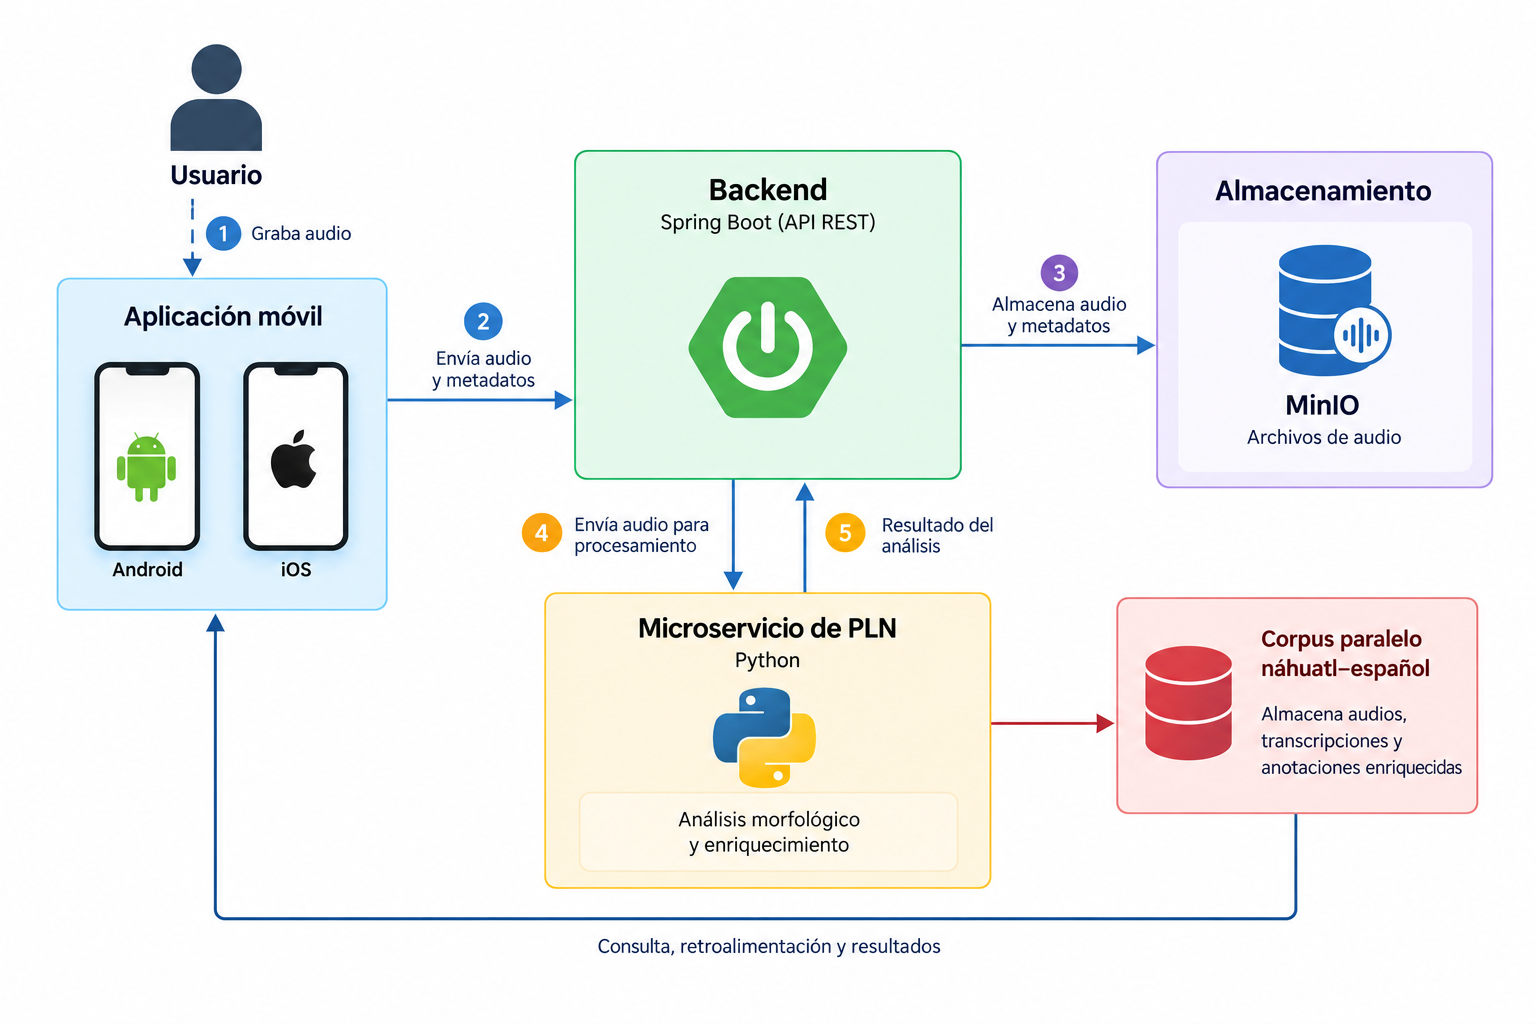
\includegraphics[width=.96\paperwidth,height=7.1cm,keepaspectratio]{assets/arquitectura.png}
  };
\end{tikzpicture}
\end{frame}
\begin{frame}[label=cronograma]{Cronograma de actividades (1/4)}
\centering
\begin{tikzpicture}[x=\linewidth,y=1cm]
  \begin{scope}
    \clip[rounded corners=6pt] (0,0) rectangle (1,5.3);
    \fill[Paper] (0,0) rectangle (1,5.3);
    \fill[NahuaGreen] (0,4.6) rectangle (1,5.3);
    \fill[NahuaGreenLight] (0,3.0) rectangle (1,4.6);
    \fill[NahuaGreenLight] (0,0.7) rectangle (1,1.4);
  \end{scope}
  \draw[NahuaGreen!25,rounded corners=6pt] (0,0) rectangle (1,5.3);
  \draw[NahuaGreen!18] (0,3.0)--(1,3.0);
  \draw[NahuaGreen!18] (0,1.4)--(1,1.4);
  \draw[NahuaGreen!18] (0,0.7)--(1,0.7);
  \node[anchor=west,text=white,font=\normalsize\bfseries] at (.03,4.95) {Actividad};
  \node[anchor=west,text=Ink,font=\fontsize{11}{14}\selectfont,align=left,text width=.94\linewidth,inner sep=0pt] at (.03,3.8) {\textbf{1.} Analizar las tecnologías de información y comunicación aplicables al desarrollo de una plataforma móvil para la construcción y enriquecimiento de un corpus paralelo náhuatl–español.};
  \node[anchor=west,text=Ink,font=\fontsize{11}{14}\selectfont,align=left,text width=.94\linewidth,inner sep=0pt] at (.03,2.2) {\textbf{2.} Analizar los métodos, técnicas y recursos lingüísticos utilizados para la recopilación, organización, transcripción y gestión de datos de corpus en lenguas de bajos recursos.};
  \node[anchor=west,text=Ink,font=\fontsize{11}{14}\selectfont,align=left,text width=.94\linewidth,inner sep=0pt] at (.03,1.05) {\textbf{3.} Redactar el capítulo 1 de la tesis.};
  \node[anchor=west,text=Ink,font=\fontsize{11}{14}\selectfont,align=left,text width=.94\linewidth,inner sep=0pt] at (.03,0.35) {\textbf{4.} Redactar el capítulo 2 de la tesis.};
\end{tikzpicture}
\end{frame}
\begin{frame}{Cronograma de actividades (2/4)}
\centering
\begin{tikzpicture}[x=\linewidth,y=1cm]
  \begin{scope}
    \clip[rounded corners=6pt] (0,0) rectangle (1,5.3);
    \fill[Paper] (0,0) rectangle (1,5.3);
    \fill[NahuaGreen] (0,4.6) rectangle (1,5.3);
    \fill[NahuaGreenLight] (0,2.7) rectangle (1,4.6);
    \fill[NahuaGreenLight] (0,0.0) rectangle (1,1.9);
  \end{scope}
  \draw[NahuaGreen!25,rounded corners=6pt] (0,0) rectangle (1,5.3);
  \draw[NahuaGreen!18] (0,2.7)--(1,2.7);
  \draw[NahuaGreen!18] (0,1.9)--(1,1.9);
  \node[anchor=west,text=white,font=\normalsize\bfseries] at (.03,4.95) {Actividad};
  \node[anchor=west,text=Ink,font=\fontsize{11}{14}\selectfont,align=left,text width=.94\linewidth,inner sep=0pt] at (.03,3.65) {\textbf{5.} Diseñar un prototipo no funcional de la aplicación móvil, considerando los principios de usabilidad, accesibilidad y experiencia de usuario para la recopilación y clasificación de registros de audio.};
  \node[anchor=west,text=Ink,font=\fontsize{11}{14}\selectfont,align=left,text width=.94\linewidth,inner sep=0pt] at (.03,2.3) {\textbf{6.} Redactar el capítulo 3 de la tesis.};
  \node[anchor=west,text=Ink,font=\fontsize{11}{14}\selectfont,align=left,text width=.94\linewidth,inner sep=0pt] at (.03,0.95) {\textbf{7.} Diseñar la arquitectura y los servicios necesarios para la recopilación, almacenamiento, organización, sincronización y gestión de los registros de audio y sus metadatos asociados.};
\end{tikzpicture}
\end{frame}
\begin{frame}{Cronograma de actividades (3/4)}
\centering
\begin{tikzpicture}[x=\linewidth,y=1cm]
  \begin{scope}
    \clip[rounded corners=6pt] (0,0) rectangle (1,5.3);
    \fill[Paper] (0,0) rectangle (1,5.3);
    \fill[NahuaGreen] (0,4.6) rectangle (1,5.3);
    \fill[NahuaGreenLight] (0,3.0) rectangle (1,4.6);
    \fill[NahuaGreenLight] (0,1.7) rectangle (1,2.35);
    \fill[NahuaGreenLight] (0,0.0) rectangle (1,1.05);
  \end{scope}
  \draw[NahuaGreen!25,rounded corners=6pt] (0,0) rectangle (1,5.3);
  \draw[NahuaGreen!18] (0,3.0)--(1,3.0);
  \draw[NahuaGreen!18] (0,2.35)--(1,2.35);
  \draw[NahuaGreen!18] (0,1.7)--(1,1.7);
  \draw[NahuaGreen!18] (0,1.05)--(1,1.05);
  \node[anchor=west,text=white,font=\normalsize\bfseries] at (.03,4.95) {Actividad};
  \node[anchor=west,text=Ink,font=\fontsize{11}{14}\selectfont,align=left,text width=.94\linewidth,inner sep=0pt] at (.03,3.8) {\textbf{8.} Desarrollar la aplicación móvil multiplataforma para la recopilación, clasificación y gestión de registros de audio destinados a la construcción y enriquecimiento del corpus paralelo náhuatl–español.};
  \node[anchor=west,text=Ink,font=\fontsize{11}{14}\selectfont,align=left,text width=.94\linewidth,inner sep=0pt] at (.03,2.675) {\textbf{9.} Redactar el capítulo 4 de la tesis.};
  \node[anchor=west,text=Ink,font=\fontsize{11}{14}\selectfont,align=left,text width=.94\linewidth,inner sep=0pt] at (.03,2.025) {\textbf{10.} Realizar la estancia académica.};
  \node[anchor=west,text=Ink,font=\fontsize{11}{14}\selectfont,align=left,text width=.94\linewidth,inner sep=0pt] at (.03,1.375) {\textbf{11.} Redactar el capítulo 5 de la tesis.};
  \node[anchor=west,text=Ink,font=\fontsize{11}{14}\selectfont,align=left,text width=.94\linewidth,inner sep=0pt] at (.03,.525) {\textbf{12.} Efectuar las correcciones necesarias en la redacción y documentación de la tesis.};
\end{tikzpicture}
\end{frame}
\begin{frame}{Cronograma de actividades (4/4)}
\centering
\begin{tikzpicture}[x=\linewidth,y=1cm]
  \begin{scope}
    \clip[rounded corners=6pt] (0,0) rectangle (1,5.3);
    \fill[Paper] (0,0) rectangle (1,5.3);
    \fill[NahuaGreen] (0,4.6) rectangle (1,5.3);
    \fill[NahuaGreenLight] (0,2.2) rectangle (1,4.6);
    \fill[NahuaGreenLight] (0,0.0) rectangle (1,1.1);
  \end{scope}
  \draw[NahuaGreen!25,rounded corners=6pt] (0,0) rectangle (1,5.3);
  \draw[NahuaGreen!18] (0,2.2)--(1,2.2);
  \draw[NahuaGreen!18] (0,1.1)--(1,1.1);
  \node[anchor=west,text=white,font=\normalsize\bfseries] at (.03,4.95) {Actividad};
  \node[anchor=west,text=Ink,font=\fontsize{11}{14}\selectfont,align=left,text width=.94\linewidth,inner sep=0pt] at (.03,3.4) {\textbf{13.} Evaluar el funcionamiento de la plataforma mediante casos de estudio como prueba de concepto, considerando la recopilación, organización y gestión de los registros de audio destinados al corpus paralelo náhuatl–español.};
  \node[anchor=west,text=Ink,font=\fontsize{11}{14}\selectfont,align=left,text width=.94\linewidth,inner sep=0pt] at (.03,1.65) {\textbf{14.} Presentar el examen TOEFL.};
  \node[anchor=west,text=Ink,font=\fontsize{11}{14}\selectfont,align=left,text width=.94\linewidth,inner sep=0pt] at (.03,0.55) {\textbf{15.} Realizar el examen de grado.};
\end{tikzpicture}
\end{frame}
\begin{frame}{Cronograma de actividades: 2027}
\centering
\begin{tikzpicture}[x=\linewidth,y=1cm]
  \node[anchor=west,text=Ink,font=\fontsize{8}{10}\selectfont] at (0,5.18) {Responsable del proyecto: Israel Alberto Huerta Fernández};
  \node[anchor=east,text=Terracotta,font=\fontsize{7}{9}\selectfont] at (1,4.86) {\rule{9pt}{6pt}\enspace Periodo programado};
  \begin{scope}
    \clip[rounded corners=5pt] (0,0) rectangle (1,4.53);
    \fill[Paper] (0,0) rectangle (1,4.53);
    \fill[NahuaGreen] (0,4.05) rectangle (1,4.53);
    \fill[NahuaGreenLight] (0,0) rectangle (.1,4.05);
    \fill[Terracotta!85!Paper] (0.1000,3.7800) rectangle (0.1750,4.0500);
    \fill[Sand!50!Paper] (.1,3.51) rectangle (1,3.7800);
    \fill[Terracotta!85!Paper] (0.1000,3.5100) rectangle (0.1750,3.7800);
    \fill[Terracotta!85!Paper] (0.1000,3.2400) rectangle (0.1750,3.5100);
    \fill[Sand!50!Paper] (.1,2.97) rectangle (1,3.2400);
    \fill[Terracotta!85!Paper] (0.1750,2.9700) rectangle (0.2500,3.2400);
    \fill[Terracotta!85!Paper] (0.2500,2.9700) rectangle (0.3250,3.2400);
    \fill[Terracotta!85!Paper] (0.2500,2.7000) rectangle (0.3250,2.9700);
    \fill[Terracotta!85!Paper] (0.3250,2.7000) rectangle (0.4000,2.9700);
    \fill[Sand!50!Paper] (.1,2.43) rectangle (1,2.7000);
    \fill[Terracotta!85!Paper] (0.3250,2.4300) rectangle (0.4000,2.7000);
    \fill[Terracotta!85!Paper] (0.4000,2.4300) rectangle (0.4750,2.7000);
    \fill[Terracotta!85!Paper] (0.4000,2.1600) rectangle (0.4750,2.4300);
    \fill[Terracotta!85!Paper] (0.4750,2.1600) rectangle (0.5500,2.4300);
    \fill[Sand!50!Paper] (.1,1.89) rectangle (1,2.1600);
    \fill[Terracotta!85!Paper] (0.4750,1.8900) rectangle (0.5500,2.1600);
    \fill[Terracotta!85!Paper] (0.5500,1.8900) rectangle (0.6250,2.1600);
    \fill[Terracotta!85!Paper] (0.6250,1.8900) rectangle (0.7000,2.1600);
    \fill[Terracotta!85!Paper] (0.7000,1.8900) rectangle (0.7750,2.1600);
    \fill[Terracotta!85!Paper] (0.6250,1.6200) rectangle (0.7000,1.8900);
    \fill[Terracotta!85!Paper] (0.7000,1.6200) rectangle (0.7750,1.8900);
    \fill[Sand!50!Paper] (.1,1.35) rectangle (1,1.6200);
    \fill[Terracotta!85!Paper] (0.4750,1.3500) rectangle (0.5500,1.6200);
    \fill[Terracotta!85!Paper] (0.5500,1.3500) rectangle (0.6250,1.6200);
    \fill[Terracotta!85!Paper] (0.6250,1.3500) rectangle (0.7000,1.6200);
    \fill[Terracotta!85!Paper] (0.7000,1.3500) rectangle (0.7750,1.6200);
    \fill[Terracotta!85!Paper] (0.7750,1.3500) rectangle (0.8500,1.6200);
    \fill[Terracotta!85!Paper] (0.8500,1.3500) rectangle (0.9250,1.6200);
    \fill[Terracotta!85!Paper] (0.7750,1.0800) rectangle (0.8500,1.3500);
    \fill[Sand!50!Paper] (.1,0.81) rectangle (1,1.0800);
    \fill[Terracotta!85!Paper] (0.7750,0.8100) rectangle (0.8500,1.0800);
    \fill[Terracotta!85!Paper] (0.8500,0.5400) rectangle (0.9250,0.8100);
    \fill[Sand!50!Paper] (.1,0.27) rectangle (1,0.5400);
    \fill[Terracotta!85!Paper] (0.7750,0.2700) rectangle (0.8500,0.5400);
    \fill[Terracotta!85!Paper] (0.8500,0.2700) rectangle (0.9250,0.5400);
    \fill[Terracotta!85!Paper] (0.9250,0.2700) rectangle (1.0000,0.5400);
    \fill[Terracotta!85!Paper] (0.9250,-0.0000) rectangle (1.0000,0.2700);
  \end{scope}
  \draw[NahuaGreen!18,line width=.25pt] (0.1000,0)--(0.1000,4.05);
  \draw[NahuaGreen!18,line width=.25pt] (0.1750,0)--(0.1750,4.05);
  \draw[NahuaGreen!18,line width=.25pt] (0.2500,0)--(0.2500,4.05);
  \draw[NahuaGreen!18,line width=.25pt] (0.3250,0)--(0.3250,4.05);
  \draw[NahuaGreen!18,line width=.25pt] (0.4000,0)--(0.4000,4.05);
  \draw[NahuaGreen!18,line width=.25pt] (0.4750,0)--(0.4750,4.05);
  \draw[NahuaGreen!18,line width=.25pt] (0.5500,0)--(0.5500,4.05);
  \draw[NahuaGreen!18,line width=.25pt] (0.6250,0)--(0.6250,4.05);
  \draw[NahuaGreen!18,line width=.25pt] (0.7000,0)--(0.7000,4.05);
  \draw[NahuaGreen!18,line width=.25pt] (0.7750,0)--(0.7750,4.05);
  \draw[NahuaGreen!18,line width=.25pt] (0.8500,0)--(0.8500,4.05);
  \draw[NahuaGreen!18,line width=.25pt] (0.9250,0)--(0.9250,4.05);
  \draw[NahuaGreen!18,line width=.25pt] (1.0000,0)--(1.0000,4.05);
  \draw[NahuaGreen!18,line width=.25pt] (0,3.7800)--(1,3.7800);
  \node[text=NahuaGreen,font=\fontsize{8}{9}\selectfont\bfseries] at (.05,3.9150) {1};
  \draw[NahuaGreen!18,line width=.25pt] (0,3.5100)--(1,3.5100);
  \node[text=NahuaGreen,font=\fontsize{8}{9}\selectfont\bfseries] at (.05,3.6450) {2};
  \draw[NahuaGreen!18,line width=.25pt] (0,3.2400)--(1,3.2400);
  \node[text=NahuaGreen,font=\fontsize{8}{9}\selectfont\bfseries] at (.05,3.3750) {3};
  \draw[NahuaGreen!18,line width=.25pt] (0,2.9700)--(1,2.9700);
  \node[text=NahuaGreen,font=\fontsize{8}{9}\selectfont\bfseries] at (.05,3.1050) {4};
  \draw[NahuaGreen!18,line width=.25pt] (0,2.7000)--(1,2.7000);
  \node[text=NahuaGreen,font=\fontsize{8}{9}\selectfont\bfseries] at (.05,2.8350) {5};
  \draw[NahuaGreen!18,line width=.25pt] (0,2.4300)--(1,2.4300);
  \node[text=NahuaGreen,font=\fontsize{8}{9}\selectfont\bfseries] at (.05,2.5650) {6};
  \draw[NahuaGreen!18,line width=.25pt] (0,2.1600)--(1,2.1600);
  \node[text=NahuaGreen,font=\fontsize{8}{9}\selectfont\bfseries] at (.05,2.2950) {7};
  \draw[NahuaGreen!18,line width=.25pt] (0,1.8900)--(1,1.8900);
  \node[text=NahuaGreen,font=\fontsize{8}{9}\selectfont\bfseries] at (.05,2.0250) {8};
  \draw[NahuaGreen!18,line width=.25pt] (0,1.6200)--(1,1.6200);
  \node[text=NahuaGreen,font=\fontsize{8}{9}\selectfont\bfseries] at (.05,1.7550) {9};
  \draw[NahuaGreen!18,line width=.25pt] (0,1.3500)--(1,1.3500);
  \node[text=NahuaGreen,font=\fontsize{8}{9}\selectfont\bfseries] at (.05,1.4850) {10};
  \draw[NahuaGreen!18,line width=.25pt] (0,1.0800)--(1,1.0800);
  \node[text=NahuaGreen,font=\fontsize{8}{9}\selectfont\bfseries] at (.05,1.2150) {11};
  \draw[NahuaGreen!18,line width=.25pt] (0,0.8100)--(1,0.8100);
  \node[text=NahuaGreen,font=\fontsize{8}{9}\selectfont\bfseries] at (.05,0.9450) {12};
  \draw[NahuaGreen!18,line width=.25pt] (0,0.5400)--(1,0.5400);
  \node[text=NahuaGreen,font=\fontsize{8}{9}\selectfont\bfseries] at (.05,0.6750) {13};
  \draw[NahuaGreen!18,line width=.25pt] (0,0.2700)--(1,0.2700);
  \node[text=NahuaGreen,font=\fontsize{8}{9}\selectfont\bfseries] at (.05,0.4050) {14};
  \draw[NahuaGreen!18,line width=.25pt] (0,-0.0000)--(1,-0.0000);
  \node[text=NahuaGreen,font=\fontsize{8}{9}\selectfont\bfseries] at (.05,0.1350) {15};
  \node[text=white,font=\fontsize{7}{8}\selectfont\bfseries] at (.05,4.29) {Actividad};
  \node[text=white,font=\fontsize{6}{7}\selectfont\bfseries,inner sep=0pt] at (0.1375,4.29) {Enero};
  \node[text=white,font=\fontsize{6}{7}\selectfont\bfseries,inner sep=0pt] at (0.2125,4.29) {Febrero};
  \node[text=white,font=\fontsize{6}{7}\selectfont\bfseries,inner sep=0pt] at (0.2875,4.29) {Marzo};
  \node[text=white,font=\fontsize{6}{7}\selectfont\bfseries,inner sep=0pt] at (0.3625,4.29) {Abril};
  \node[text=white,font=\fontsize{6}{7}\selectfont\bfseries,inner sep=0pt] at (0.4375,4.29) {Mayo};
  \node[text=white,font=\fontsize{6}{7}\selectfont\bfseries,inner sep=0pt] at (0.5125,4.29) {Junio};
  \node[text=white,font=\fontsize{6}{7}\selectfont\bfseries,inner sep=0pt] at (0.5875,4.29) {Julio};
  \node[text=white,font=\fontsize{6}{7}\selectfont\bfseries,inner sep=0pt] at (0.6625,4.29) {Agosto};
  \node[text=white,font=\fontsize{6}{7}\selectfont\bfseries,inner sep=0pt] at (0.7375,4.29) {Septiembre};
  \node[text=white,font=\fontsize{6}{7}\selectfont\bfseries,inner sep=0pt] at (0.8125,4.29) {Octubre};
  \node[text=white,font=\fontsize{6}{7}\selectfont\bfseries,inner sep=0pt] at (0.8875,4.29) {Noviembre};
  \node[text=white,font=\fontsize{6}{7}\selectfont\bfseries,inner sep=0pt] at (0.9625,4.29) {Diciembre};
  \draw[NahuaGreen!30,rounded corners=5pt] (0,0) rectangle (1,4.53);
\end{tikzpicture}
\end{frame}
\begin{frame}[label=conclusiones]{Conclusiones}
\begin{itemize}[<+->]
\setlength{\itemsep}{.55cm}
\item La revisión realizada identifica la \textbf{\color{Terracotta}disponibilidad limitada} de recursos lingüísticos computacionales para \textbf{\color{NahuaGreen}lenguas de bajos recursos}.
\item La \textbf{\color{NahuaGreen}diversidad lingüística del náhuatl} forma parte de las consideraciones necesarias para la \textbf{\color{Terracotta}construcción y enriquecimiento del corpus}.
\item Los antecedentes revisados proporcionan elementos para abordar la \textbf{\color{NahuaGreen}recopilación, organización}, \textbf{\color{Terracotta}análisis y validación} de datos lingüístico.
\end{itemize}
\end{frame}
\begin{frame}[label=compromisos]{Compromisos a futuro}
\begin{itemize}[<+->]
\setlength{\itemsep}{.55cm}
\item Cumplir en tiempo y forma con las actividades del cronograma.
\item Atender en tiempo y forma las observaciones realizadas al anteproyecto de tesis por parte del jurado.
\item Concluir en tiempo y forma el anteproyecto de tesis.
\end{itemize}
\end{frame}
\begin{frame}[t,label=referencias]{Referencias}
\framesubtitle{1/3}
\fontsize{9}{10.5}\selectfont
\begin{thebibliography}{99}
\setlength{\itemsep}{0.25cm}
\bibitem{kmp}
JetBrains, ``Kotlin Multiplatform.'' [En línea]. Disponible en: \url{https://kotlinlang.org/docs/multiplatform.html}.

\bibitem{compose}
JetBrains, ``Compose Multiplatform.'' [En línea]. Disponible en: \url{https://www.jetbrains.com/lp/compose-multiplatform/}.

\bibitem{flutter}
Flutter, ``Flutter Documentation.'' [En línea]. Disponible en: \url{https://docs.flutter.dev/}.

\bibitem{rn}
Meta, ``React Native Documentation.'' [En línea]. Disponible en: \url{https://reactnative.dev/}.

\setcounter{bibliographycontinuation}{\value{enumiv}}
\end{thebibliography}
\end{frame}
\begin{frame}[t]{Referencias}
\framesubtitle{2/3}
\fontsize{9}{10.5}\selectfont
\begin{thebibliography}{99}
\setlength{\itemsep}{0.25cm}
\setcounter{enumiv}{\value{bibliographycontinuation}}
\bibitem{maui}
Microsoft, ``.NET MAUI Documentation.'' [En línea]. Disponible en: \url{https://learn.microsoft.com/dotnet/maui/}.

\bibitem{spring}
Spring, ``Spring Boot.'' [En línea]. Disponible en: \url{https://spring.io/projects/spring-boot}.

\bibitem{mongo}
MongoDB, ``MongoDB Documentation.'' [En línea]. Disponible en: \url{https://www.mongodb.com/docs/}.

\bibitem{minio}
MinIO, ``MinIO Documentation.'' [En línea]. Disponible en: \url{https://min.io/}.

\setcounter{bibliographycontinuation}{\value{enumiv}}
\end{thebibliography}
\end{frame}
\begin{frame}[t]{Referencias}
\framesubtitle{3/3}
\fontsize{9}{10.5}\selectfont
\begin{thebibliography}{99}
\setlength{\itemsep}{0.25cm}
\setcounter{enumiv}{\value{bibliographycontinuation}}
\bibitem{hf}
Hugging Face, ``Transformers Documentation.'' [En línea]. Disponible en: \url{https://huggingface.co/docs/transformers/}.

\bibitem{scrum}
K. Schwaber y J. Sutherland, ``The Scrum Guide,'' 2020. [En línea]. Disponible en: \url{https://scrumguides.org/}.

\bibitem{kaggle}
Kaggle, ``Datasets.'' [En línea]. Disponible en: \url{https://www.kaggle.com/datasets}.

\setcounter{bibliographycontinuation}{\value{enumiv}}
\end{thebibliography}
\end{frame}
\begin{frame}[plain]\begin{center}\vspace{2cm}{\Huge\bfseries\color{NahuaGreen}Gracias}\par\vspace{.25cm}{\color{Terracotta}\rule{1.4cm}{1.2pt}}\par\vspace{.3cm}{\Large\color{NahuaDark}¿Preguntas?}\end{center}\end{frame}
\end{document}
